\documentclass{emulateapj}
\newcommand{\beq}{\begin{equation}}
\newcommand{\eeq}{\end{equation}}
\newcommand{\hyd}    {{\rm H}}
\newcommand{\vobs}{v_{\rm obs}}
\newcommand{\hi}{H{\sc i}~}
\newcommand{\hii}{H{\sc ii}~}
\newcommand{\hia}{H{\sc i}}
\newcommand{\hiia}{H{\sc ii}}

\usepackage[colorlinks,urlcolor=blue,citecolor=blue,linkcolor=blue]{hyperref}
\usepackage{gensymb}
\usepackage{amsmath}
\usepackage{color}
%\usepackage{appendix}
\usepackage[titletoc,title]{appendix}


\makeatletter
\setlength{\@fptop}{0pt}
\setlength{\@fpbot}{0pt}
\setlength{\@fpsep}{0pt}
\makeatother

\newcommand{\citei}[1]{\citeauthor{#1} \citeyear{#1}}
\newcommand{\unit}[1]{\textrm{ #1}}
\newcommand{\kms}{km ${\rm s^{-1}}$}
\newcommand{\kmsa}{km ${\rm s^{-1}}$}
\newcommand{\citeia}[2]{\citeauthor{#1}~(\citeyear{#1};~#2)}

\newcommand\reye{\mathrel{Re}}
\newcommand\reym{\mathrel{Rm}}

\renewcommand{\topfraction}{0.85}
\renewcommand{\textfraction}{0.1}
\renewcommand{\floatpagefraction}{0.75}

\begin{document}

\title{The Weakly Nonlinear Saturation of the Magnetorotational Instability}
\author{Clark, S.E.\altaffilmark{1}}
\author{Oishi, J.S. \altaffilmark{2,}\altaffilmark{3}}
\author{Mac Low, M.-M.\altaffilmark{1,}\altaffilmark{2}}
\altaffiltext{1}{Department of Astronomy, Columbia University, New York, NY} 
\altaffiltext{2}{Department of Astrophysics, American Museum of Natural History, New York, NY}
\altaffiltext{3}{Department of Physics, SUNY Farmingdale}


\begin{abstract}
The magnetorotational instability (MRI) is a fundamental process of accretion disk physics, but its saturation mechanism remains poorly understood. We present an analytic analysis of the nonideal MRI in the weakly nonlinear regime -- that is, when the MRI system is just unstable to its most unstable mode. 
\end{abstract}



\section{Introduction}

For matter to accrete from a disk onto a central object, angular momentum must be transported radially outward in the disk. The transport mechanism is likely turbulent (\citei{Shakura:1973wg}). Since its discovery by \citeauthor{Chandrasekhar:1960wh} (\citeyear{Chandrasekhar:1960wh}) and subsequent rediscovery by \citeauthor{Balbus:1991vs} (\citeyear{Balbus:1991vs}), the MRI remains the leading explanation for rapid angular momentum transport in astrophysical disks. The instability arises when a differentially rotating disk is threaded by a vertical magnetic field. The presence of the magnetic field destabilizes the disk gas, driving turbulence and angular momentum transport.

The MRI evolves via a period of linear growth, followed by nonlinear saturation. The nonlinear evolution of the MRI is a complex process, and an understanding of the mechanism by which the MRI saturates remains elusive. Most previous works on MRI saturation have studied the problem in simulation. Indeed, only a few works have tackled MRI saturation analytically. We briefly summarize a few of these analytic contributions.

%examples of simulations papers
%more mention of other analytic works

This work builds on the investigations of \citeauthor{Umurhan:2007hs} (\citeyear{Umurhan:2007hs}; see also \citei{Umurhan:2007dz}), who first conducted an analytic analysis of the MRI in the weakly nonlinear regime. 

We develop this investigation with the goal of providing a rigorous analytical framework that will be used to make predictions for laboratory MRI experiments. Observing MRI in a laboratory setting would open a new avenue for studying MRI dynamics and saturation. In recent years much experimental progress has been made, although no experiment has yet yielded a confirmed detection. Of most immediate interest to this work is the Princeton Plasma Physics Laboratory (PPPL) MRI experiment, which has a design roughly analogous to the set-up investigated here (see \S\ref{setup} for further details). The Madison plasma dynamo experiment is a multi-purpose plasma device which may be a vehicle for MRI studies in the near future (\citei{Cooper:2013to}). The helical MRI, an instability related to the standard MRI but easier to excite in the laboratory, is the focus of the Potsdam Rossendorf Magnetic Instability Experiment (PROMISE) in Dresden. PROMISE has already detected helical MRI in the laboratory (e.g. \citei{Stefani:2006iv}), and we discuss possible applications of our framework to the helical MRI in \S\ref{discussion}. A spherical Couette experiment claimed to have detected MRI in 2004 (\citeauthor{Sisan:2004ig}), but most likely detected unrelated MHD instabilities instead (\citei{Hollerbach:2009ig}; \citei{Gissinger:2011td}).

The focus of this work is the weakly nonlinear regime of the MRI. This is where the initial linear growth phase of the instability begins to give way to nonlinear saturation. Weakly nonlinear analysis is the perturbation analysis of a system that is just unstable to its most unstable mode. The system in its marginal state, when the most unstable mode neither grows nor decays, is tuned slightly into instability. This excites a band of wavemodes around the most unstable mode, which interact nonlinearly. In order to track the evolution of the system on both rapid and slow scales, we conduct a formal multiscale analysis. 

%relation to hTC and R-B
%explanation of WNA

\section{Set-Up}


\begin{figure}[h!]
\centering
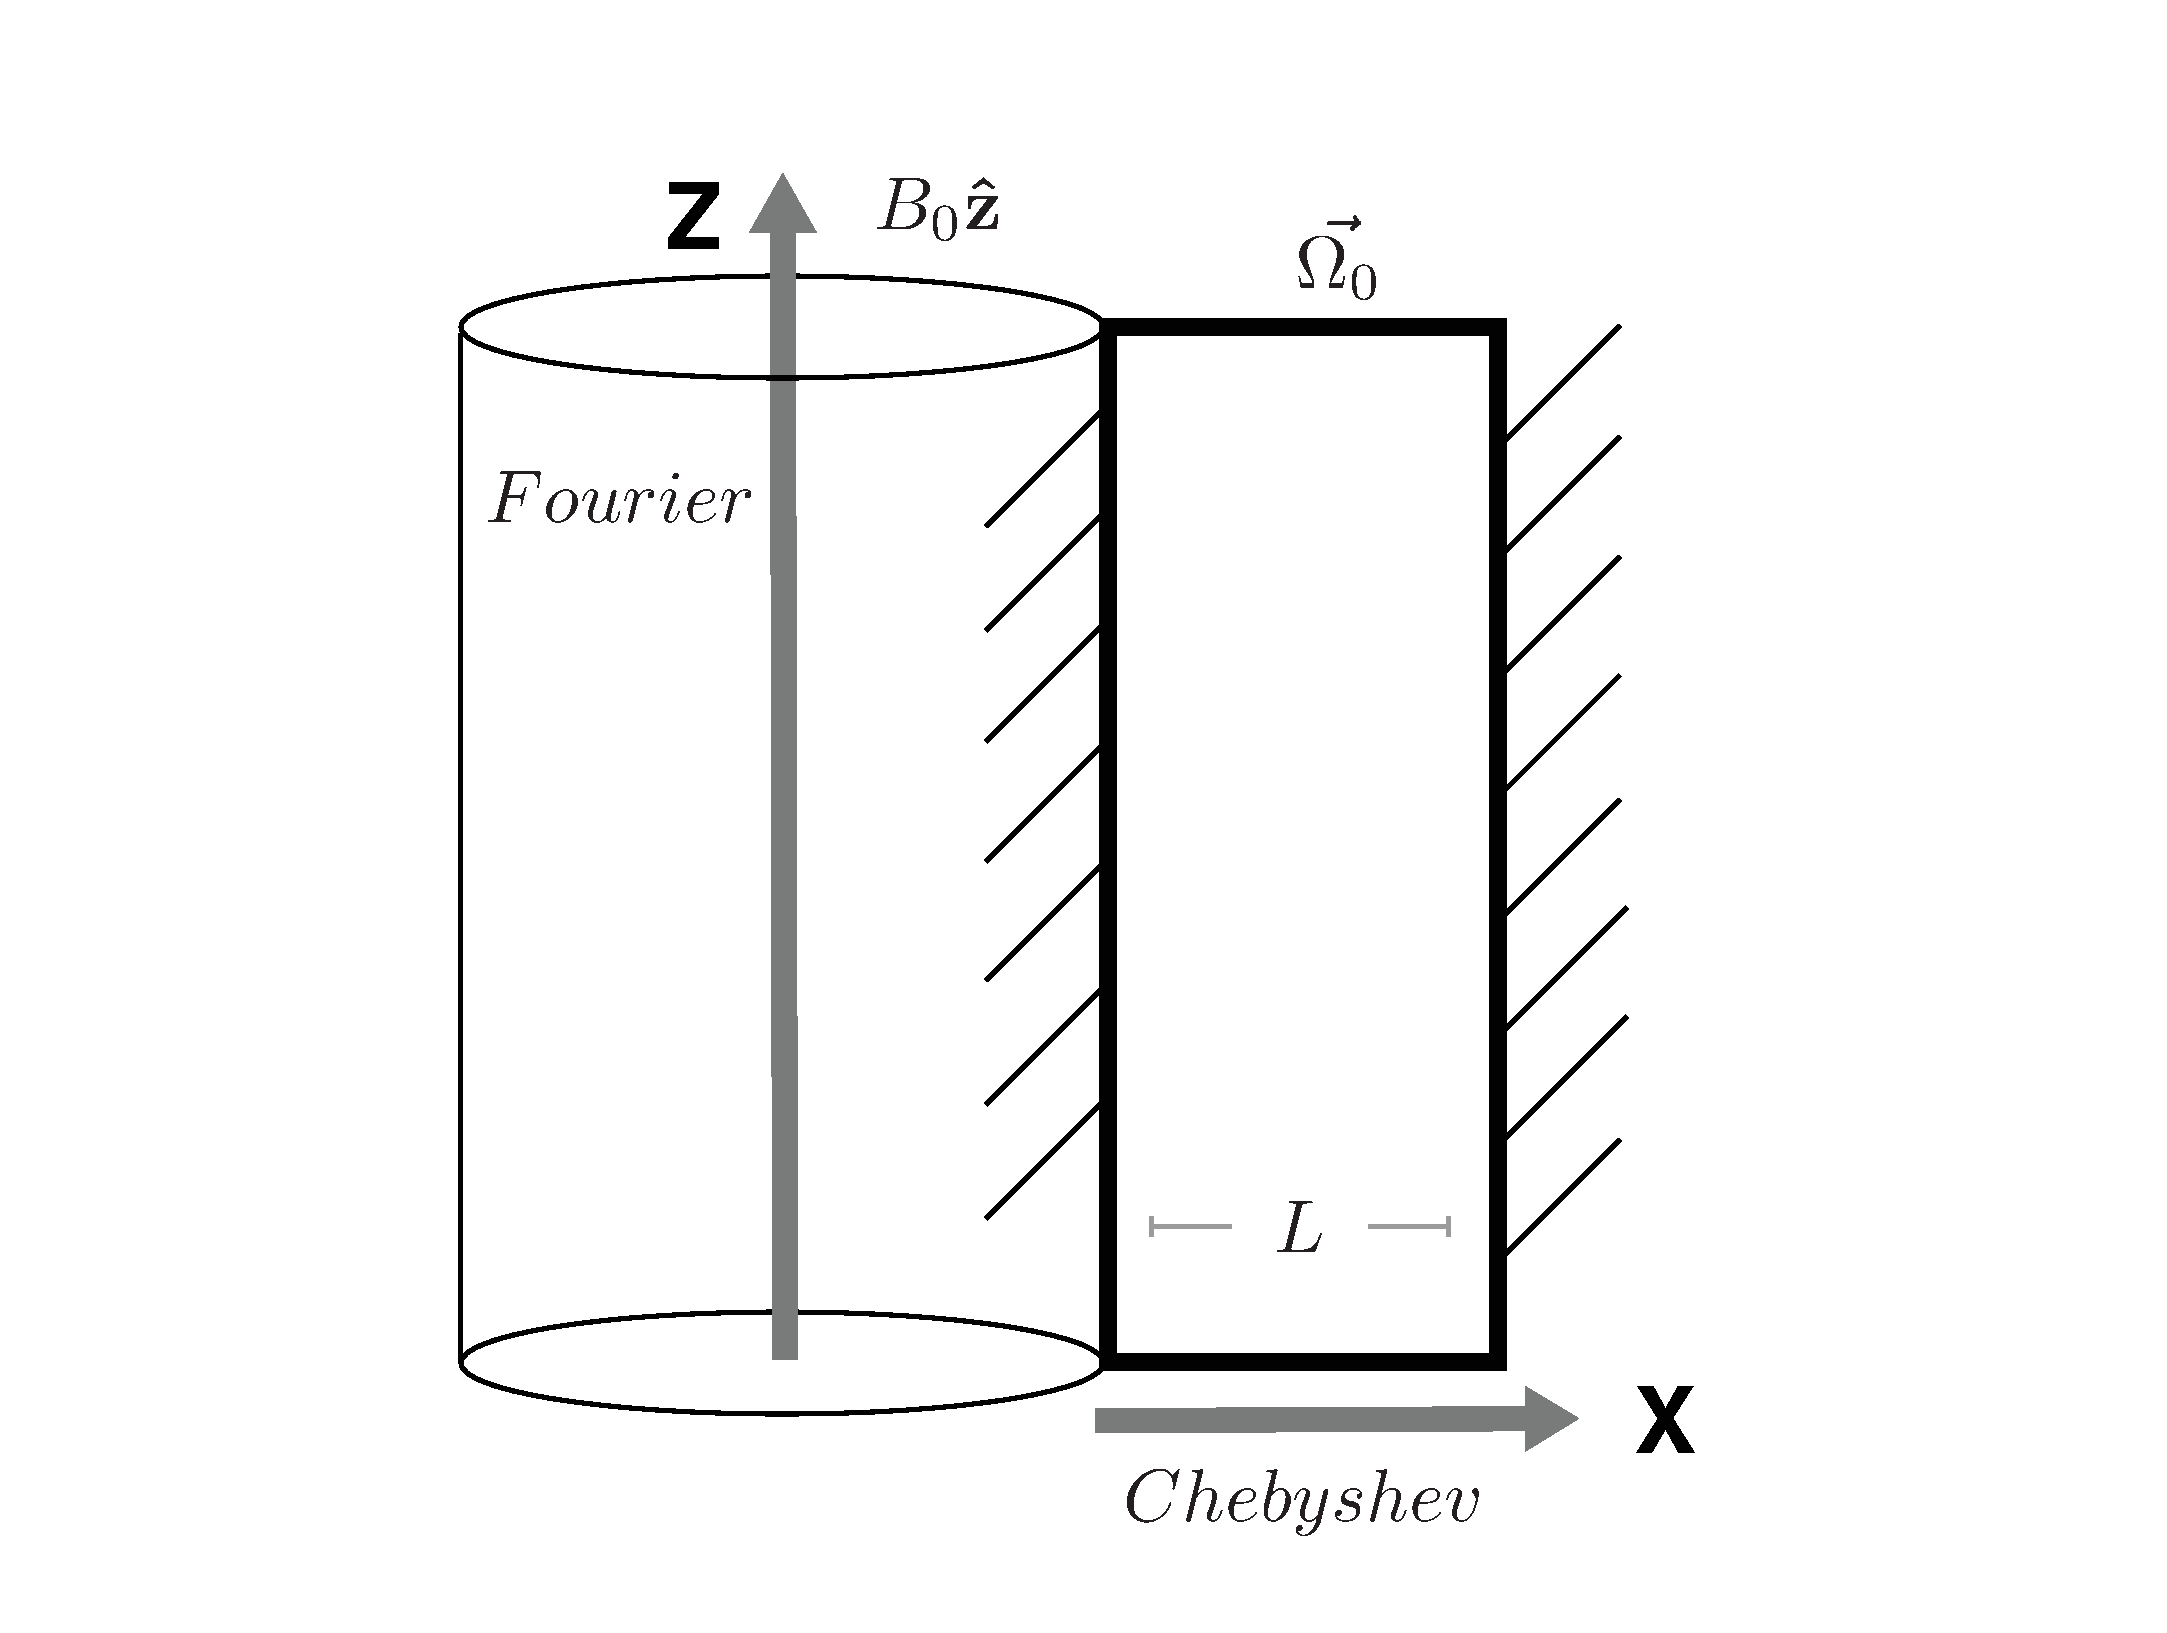
\includegraphics[trim=5cm 0cm 0cm 0cm, scale=.35]{setup_diagram.eps}
\caption{Schematic diagram of our set-up, an axisymmetric magnetized Taylor Couette flow. We investigate a 2D slice of the X-Z (radial-vertical) plane. Our domain is the bolded black box, of width L. The radial dimension is solved with a basis of Chebyshev polynomials, and the vertical dimension is solved on a Fourier basis (see \S\ref{discussion}.) }\label{setup}
\end{figure}

We analyze a magnetized Taylor Couette flow, representing a differentially rotating, conducting fluid between two cylinders which are driven at different speeds. We initialize an angular velocity profile which decreases outward from the axis of rotation, and a weak vertical magnetic field. These are the only two conditions required to excite MRI. The differential rotation profile is

\beq
\Omega\left(r\right) \propto \Omega_0\left(\frac{r}{r_0}\right)^{-q},
\eeq

where $q$, the shear parameter, is $3/2$ for Keplerian rotation. The initial background magnetic field is

\beq
\mathbf{B} = B_0 \hat{z},
\eeq

a constant, vertical field.

We analyze this system in the thin-gap regime, where the channel is radially narrow. Formally, this means

\beq
thin gap equation,
\eeq

the width of the channel is small compared to its distance from the center of rotation. The imposition of the thin-gap approximation eliminates channel modes, the axisymmetric MRI modes that are exact solutions of the incompressible MRI in the shearing box approximation (\citei{Goodman:1994ul}). Implications of this approximation are discussed further in \S\ref{discussion}.

Our domain is designed to be relevant to the design of the PPPL MRI experiment (see \S\ref{discussion} for further discussion). We use periodic vertical boundary conditions. On the radial boundaries of our domain --  the inner and outer cylinders -- we apply no-slip, perfectly conducting boundary conditions. The choice of boundary conditions dictates the functional bases on which our system is spectrally solved. This is explained further in \S\ref{wna}. A diagram of our set-up is shown in Figure \ref{setup}.


\section{Weakly Nonlinear Analysis}\label{wna}

We solve the equations of non-ideal, axisymmetric, incompressible magnetized Taylor Couette flow. We solve the momentum equation,

\beq\label{momentum}
\partial_t \mathbf{u} \, + \, \mathbf{u} \cdot \nabla \mathbf{u} \, = 
\eeq

$\, -\frac{1}{\rho}\nabla P \, - \, \nabla\Phi \, + \, \frac{1}{\rho} \left(\mathbf{J}\times\mathbf{B}\right) \, + \, \nu\nabla^2 \mathbf{u} \, - \, 2\mathbf{\Omega} \times \mathbf{u} \, - \, \mathbf{\Omega} \times \left(\mathbf{\Omega} \times \mathbf{r} \right)$


and the induction equation,

\beq\label{induction}
\partial_t \mathbf{B} = \nabla \times \left(\mathbf{u} \times \mathbf{B}\right) + \eta\nabla^2\mathbf{B}.
\eeq

Equations \ref{momentum} and \ref{induction} are subject to the magnetic solenoid and incompressibility constraints,

\beq
\nabla \cdot \mathbf{B} = 0
\eeq

and

\beq
\nabla \cdot \mathbf{u} = 0.
\eeq

We perturb the fluid quantities with three-dimensional, axisymmetric perturbations. We nondimensionalize the equations according to [...]
The fluid symbols $\mathbf{u}$, $\mathbf{B}$, etc. will henceforth be used to refer to the perturbed quantities.

We define the flux function $A$ and streamfunction $\Psi$. $A$ is the familiar two-dimensional vector potential. $A$ and $\Psi$ are scalar fields defined as the curl of the magnetic field and velocity, respectively, and so automatically satisfy our constraints.

$A$ is thus related to the magnetic field as

\beq
\mathbf{B} \, = \, \left[\begin{matrix}
\partial_zA \\
B_{y} \\
-\partial_xA \\
\end{matrix}\right],\eeq \\

and $\mathbf{\Psi}$ is defined analogously.

The perturbed, nondimensionalized equations which will be the focus of this equation are as follows:

Our final equation set is: 

\begin{multline}
\label{eqset1}
\partial_t \nabla^2 \Psi \, + \, J\left(\Psi, \nabla^2 \Psi\right) \, - \, 2 \partial_z u_{1y} \, = \\
\, \frac{2}{\beta} B_0 \partial_z \nabla^2 A \, + \, \frac{2}{\beta}J\left(A, \nabla^2 A \right) \, + \, \frac{1}{\reye}\nabla^4 \Psi
\end{multline}

\begin{multline}
\label{eqset2}
\partial_t u_{1y} \, + \, J\left(\Psi, u_{1y}\right) \, + \, \left(2 - q\right) \Omega_0 \partial_z \Psi \, = \\
\, \frac{2}{\beta}B_0\partial_z B_{1y} \, + \, \frac{2}{\beta} J\left(A, B_{1y}\right) \, + \, \frac{1}{\reye} \nabla^2 u_{1y}
\end{multline}

\begin{multline}
\label{eqset3}
\partial_t A \, = \, B_0 \partial_z \Psi \, + \, J\left(A, \Psi\right) \, + \, \frac{1}{\reym} \nabla^2 A
\end{multline}

\begin{multline}
\label{eqset4}
\partial_t B_{1y} \, = \, B_0 \partial_z u_{1y} \, + \, J\left(A, u_{1y}\right) \, - \, J\left(\Psi, B_{1y}\right) \, \\
+ \, \frac{1}{\reym} \nabla^2 B_{1y}  \, - \, q \Omega_0 \partial_z A
\end{multline}

Where $J$ is the Jacobian operator, 
\beq
J\left(f, g\right) \equiv \partial_z f\partial_x g - \partial_x f \partial_z g.
\eeq  

Note that working in terms of the flux function raises the order of the first momentum equation.

The weakly nonlinear regime is where the MRI system is nonlinearly unstable to only the most unstable mode of the linear solution. We find the marginal state, where the most unstable linear MRI mode neither grows nor decays, for a given set of dimensionless parameters. 

$B_0$ appears in Equations \ref{eqset1} - \ref{eqset4} because it is the nondimensionalized background field strength. That is, $B = B_0 \equiv 1$. In order to study our system in the weakly nonlinear regime, we tune the background magnetic field down away from stability (recall that stronger vertical fields stabilize the MRI). We do so by substituting $B = B_0\left(1 - \epsilon^2\right)$. The degree of departure from the marginal state is measured by the small parameter $\epsilon$. An $\mathcal{O}\left(\epsilon^2\right)$ weakening of the background magnetic field destabilizes a band of wave modes with width of $\mathcal{O}\left(\epsilon\right)$, which interact nonlinearly.

The destabilizing substitution is made, and Equations \ref{eqset1} - \ref{eqset4} are rewritten such that the fluid variables are contained in a state vector $\mathbf{V} = \left[\Psi, u_y, A, B_y\right]^\mathrm{T}$. This yields the following system of equations.

\beq
\mathcal{D}\partial_t \mathbf{V} + \mathbf{N} = \mathcal{L} \mathbf{V} - \epsilon^2\partial_z\mathcal{X} \mathbf{V} - \epsilon^2 \partial_z^3 \mathcal{L}_3\mathbf{V}
\eeq

Where $\mathcal{L} \equiv \mathcal{L}_0 + \mathcal{L}_1\partial_z + \mathcal{L}_2\partial_z^2 + \mathcal{L}_3\partial_z^3 + \mathcal{L}_4\partial_z^4$ \\

And:

\beq
\mathcal{D} = \left[\begin{matrix}
\nabla^2 & 0 & 0 & 0 \\
0 & 1& 0 & 0 \\
0 & 0 & 1 & 0\\
0 & 0 & 0 & 1 \\
\end{matrix}\right]
\eeq

\beq
\mathcal{L}_0 = \left[\begin{matrix}
\frac{1}{\reye}\partial_x^4 & 0 & 0 & 0 \\
0 & \frac{1}{\reye}\partial_x^2 & 0 &0 \\
0 & 0 & \frac{1}{\reym}\partial_x^2 & 0 \\
0 & 0 & 0 & \frac{1}{\reym}\partial_x^2 \\ \end{matrix}\right]
\eeq

\beq
\mathcal{L}_1 = \left[\begin{matrix}
0 & 2 & \frac{2}{\beta}\partial_x^2 & 0 \\
(\Omega_0 - 2)q & 0 & 0 & \frac{2}{\beta} \\
1 & 0 & 0 & 0 \\
0 & 1 & -q\Omega_0 & 0 \\ \end{matrix}\right] 
\eeq

\beq
\mathcal{L}_2 = \left[\begin{matrix}
2\frac{1}{\reye} \partial_x^2 & 0 & 0 & 0 \\
0 & \frac{1}{\reye} & 0 & 0 \\
0 & 0 & \frac{1}{\reym} & 0 \\
0 & 0 & 0 & \frac{1}{\reym} \\ \end{matrix}\right]
\eeq

\beq
\mathcal{L}_3 = \left[\begin{matrix}
0 & 0 & \frac{2}{\beta} & 0 \\
0 & 0 & 0 & 0 \\
0 & 0 & 0 & 0 \\
0 & 0 & 0 & 0 \\ \end{matrix} \right]
\eeq

\beq
\mathcal{L}_4 = \left[\begin{matrix}
\frac{1}{\reye} & 0 & 0 & 0 \\
0 & 0 & 0 & 0 \\
0 & 0 & 0 & 0 \\
0 & 0 & 0 & 0 \\ \end{matrix}\right] 
\eeq

\beq
\mathcal{X} = \left[\begin{matrix}
0 & 0 & \frac{2}{\beta}\partial_x^2 & 0 \\
0 & 0 & 0 & \frac{2}{\beta} \\
1 & 0 & 0 & 0 \\
0 & 1 & 0 & 0 \\ \end{matrix} \right]. 
\eeq


We conduct a formal multiscale analysis. Our perturbations are characterized in terms of fast and slow-moving variables, in order to simultaneously track their evolution on fast and slow scales. The relative scalings of the fast and slow scales are determined as follows. When our four equations are linearized for axisymmetric perturbations of the form $e^{\sigma t + i k_x x + i k_z z}$, we can derive the linear dispersion relation, which is fourth order in $\sigma$. The fast and slow variables are then defined such that each of the temporal and spatial eigenvalues appear at the same lowest order in the linear dispersion relation. The scalings are: 

\beq
X \equiv \epsilon x,  \, \, Y \equiv \epsilon y, \, \, Z \equiv \epsilon z, \, \, T \equiv \epsilon^2 t
\eeq

Note that these are the same scalings as apply to Rayleigh-B\'enard convection and hydrodynamic Taylor Couette flow. Each operator is expanded to reflect these scalings -- for instance, $\partial_z$ becomes $\partial_z + \epsilon\partial_Z$. 

The multiple scale dependencies of our solution are encoded into an ansatz for the linear MRI solution at marginality,

\beq
\label{V1_ansatz}
\mathbf{V_1} = \alpha(T, Z) \mathbb{V}_{11}(x) e^{i k_c z} + c.c.,
\eeq

where $\alpha$ is a slowly-varying amplitude equation. The $x$ dependence is contained in $\mathbb{V}_{11}$, and must be solved for subject to the radial boundary conditions. The periodic vertical boundary conditions allow us to posit the $z$ dependence, where $k_c$ is the value of the vertical wavenumber at marginality. 

Because we investigate the system at marginality, where the growth rate $\sigma = 0$, the $\partial_t$ terms drop out. Thus after the multiscale expansion our system becomes

\begin{multline}
\label{multiscale_system}
\epsilon^2 \mathcal{D}\partial_T\mathbf{V} \, + \, \mathbf{N} \, = \, \mathcal{L}\mathbf{V} \, + \, \epsilon\widetilde{\mathcal{L}}_1\partial_Z\mathbf{V} \, + \, \epsilon^2\widetilde{\mathcal{L}}_2\partial_Z^2\mathbf{V} \, \\
 - \, \epsilon^2\partial_z\mathcal{X}\mathbf{V} \, - \, \epsilon^2\partial_z^3\mathcal{L}_3\mathbf{V} \, + \, \mathcal{O}(\epsilon^3)
\end{multline}

Where

\beq
\widetilde{\mathcal{L}}_1 = \mathcal{L}_1 + 2\mathcal{L}_2\partial_z + 3\mathcal{L}_3\partial_z^2 + 4\mathcal{L}_4\partial_z^3
\eeq

\beq
\widetilde{\mathcal{L}}_2 = \mathcal{L}_2 + 3\mathcal{L}_3\partial_z + 6\mathcal{L}_4\partial_z^2
\eeq


% perturbation expansion
The state vector is expanded in orders of $\epsilon$:

\beq
\label{pert_exp}
\mathbf{V} = \epsilon\mathbf{V_1} + \epsilon^2\mathbf{V_2} + \epsilon^3\mathbf{V_3} + ...
\eeq

Substituting Equation \ref{pert_exp} into Equation \ref{multiscale_system} yields the perturbed, expanded equations. We solve these successively in increasing orders of $\epsilon$.

To $\mathcal{O}(\epsilon)$, we have

\beq
\label{ordere}
\mathcal{L}\mathbf{V_1} = 0
\eeq

To $\mathcal{O}(\epsilon^2)$: 

\beq
\label{ordere2}
\mathcal{L}\mathbf{V_2} \, = \, \mathbf{N_2} \, - \, \widetilde{\mathcal{L}}_1 \partial_Z \mathbf{V_1}
\eeq

To $\mathcal{O}(\epsilon^3)$: 

\begin{multline}
\label{ordere3}
\mathcal{D}\partial_T \mathbf{V_1} \, + \, \mathbf{N_3} \, = \, \mathcal{L} \mathbf{V_3} \, + \, \widetilde{\mathcal{L}}_1\partial_Z\mathbf{V_2} \, + \, \widetilde{\mathcal{L}}_2\partial_Z^2\mathbf{V_1} \, \\
- \partial_Z\mathcal{X}\mathbf{V_1} \, - \partial_z^3\mathcal{L}_3\mathbf{V_1}
\end{multline}

The $\mathcal{O}(\epsilon)$ equation is the equation for the linear MRI at marginality. This is the equation that is solved to find the $\mathbb{V}_{11}$ component of Equation \ref{V1_ansatz}. 

The partial differential equations that comprise Equations \ref{ordere} to \ref{ordere3} are solved in succession subject to no-slip, perfectly conducting radial boundary conditions, defined as:

\beq
\Psi = \partial_x \Psi = u_y = A = \partial_x B_y = 0
\eeq

The practical advantage of our ansatz construction (Equation \ref{V1_ansatz}) is clear: the separable x-dependence means that the radial boundary conditions are solved in only one dimension. Thus our analytical framework is able to side-step many of the resolution issues faced by multidimensional simulations. We are able to resolve even significant structure in the boundary layers of our domain, because we need only resolve it in one dimension. We solve the radial component of each equation using the open source pseudospectral code Dedalus (Burns et al., in prep). We compute the radial components on a grid of Chebyshev polynomials, as is appropriate for bounded one-dimensional domains (e.g. \citei{Boyd:2001aa}). 

We solve the system up to $\mathcal{O}(\epsilon^3)$ in order to close the solution at $\mathcal{O}(\epsilon^2)$. 

To find a bounded solution at each order, we eliminate secular terms -- terms which are resonant with solutions to the homogenous equation, and cause the solution to grow without bound. The elimination of secular terms requires enforcement of solvability criteria, which arise as a consequence of the Fredholm alternative (e.g. Guenther \& Lee 1988). The solvability criterion is found by forcing the inner product of the equation with its adjoint homogenous solution to be zero. For instance, Equation \ref{ordere2} contains a term $\widetilde{\mathcal{L}}_1 \partial_Z \mathbf{V_1}$ that is resonant with $e^{i k_c z}$. Because the adjoint homogenous equation

\beq
\mathcal{L}^\dagger \mathbf{V}^\dagger = 0
\eeq

has a nontrivial solution, the solvability criterion

\beq
\left< \mathbf{V}^\dagger \cdot \widetilde{\mathcal{L}}_1 \partial_Z \mathbf{V_1}\right> = 0 
\eeq

must be satisfied in order for Equation \ref{ordere2} to have a solution. In the above, 

\beq
\mathbf{V}^\dagger = \mathbb{V}^\dagger(x) e^{i k_c z} + c.c.
\eeq

where, again, $\mathbb{V}^\dagger$ contains the radial contribution. The elimination of this inner product must also be enforced the terms in Equation \ref{ordere3} that are resonant with $e^{i k_c z}$, yielding

\beq
\label{ampeq1}
a \partial_T \alpha \, + \, c \alpha \left|\alpha^2\right| \, + \, \widetilde{c} \alpha \partial_Z \beta \, = \, - b \partial_Z \alpha \, + \, h \partial_Z^2 \alpha \, + \, g i k_c^3 \alpha
\eeq

Where

\beq
\begin{split}
a & \equiv \left< \mathbb{V}^\dagger \cdot \mathcal{D}\mathbb{V}^*_{11}\right> \\
c & \equiv \left< \mathbb{V}^\dagger \cdot \mathbf{N}^*_{31}\right> \\
\widetilde{c} & \equiv \left< \mathbb{V}^\dagger \cdot \widetilde{\mathbf{N}}^*_{31}\right> \\
b & \equiv \left< \mathbb{V}^\dagger \cdot \left(\mathcal{X}\mathbb{V}_{11}\right)^* \right> \\
h & \equiv \left< \mathbb{V}^\dagger \cdot \left(\widetilde{\mathcal{L}}_2\mathbb{V}_{11} \, - \, \widetilde{\mathcal{L}}_1\mathbb{V}_{21} \right)^* \right> \\
g & \equiv \left< \mathbb{V}^\dagger \cdot \mathcal{L}_{3} \mathbb{V}_{11} \right> \\
\end{split}
\eeq

Equation \ref{ampeq1} is an amplitude equation -- a function of the slow variables $Z$ and $T$. We solve this initial value problem using Dedalus to obtain the asymptotic behavior of $\alpha$. This is the saturation amplitude.

\section{Results}

We conduct a full study of the MRI parameter space, focussed on the behavior with changing magnetic Prandtl number ($\mathrm{Pm} \equiv \frac{\mathrm{Rm}}{\mathrm{Re}} \equiv \frac{\nu}{\eta}$). In protoplanetary disks, as well as in liquid metal MRI experiments, the magnetic Prandtl number can be very small ($\mathrm{Pm} \sim 10^{-6}$). The scale separations caused by these large ratios of diffusivity to viscosity render the small Prandtl number regime inaccessible to simulations. This analytic formulation allows us to explore the behavior down to magnetic Prandtl numbers of [....].


\begin{figure*}[h!]
\centering
\includegraphics[scale=0.5]{allorders_velocity.eps}
\caption{First order (left) and second order (right) velocity perturbations. Streamlines represent velocity in the vertical-radial plane, where thicker streamlines correspond to faster speeds. The colorbar represents azimuthal velocity.}
\end{figure*}

\begin{figure*}[h!]
\centering
\includegraphics[scale=0.5]{allorders_Bfield.eps}
\caption{First order (left) and second order (right) velocity perturbations. Streamlines represent velocity in the vertical-radial plane, where thicker streamlines correspond to faster speeds. The colorbar represents azimuthal velocity.}
\end{figure*}

\section{Discussion}\label{discussion}

Our domain is designed to be relevant to the design of the Princeton Plasma Physics Laboratory (PPPL) MRI experiment (\citei{Ji:2001kd}). A challenge for all MRI experiments is to reduce all extraneous flows which may stabilize the MRI or obscure its detection. In particular, care must be taken to mitigate meridional flows introduced by the endcaps of the experimental apparatus. The PPPL MRI experiment employs a novel design using concentric, differentially rotating rings as endcaps (\citei{Schartman:2009df}). In this investigation, we use periodic vertical boundary conditions, so our set-up represents an idealized domain where endcap contamination does not exist. Future work will address specifically our predictions for the PPPL MRI experiment.

We compute the solutions to our derived equations pseudospectrally, using Dedalus. One advantage to using Dedalus for these computations is that the code can compute the evolution of the fully nonlinear MRI system on the same Fourier/Chebyshev grid. This allows us to directly compare simulation and theory. 

% Jeff's sims!!!!!

This work analyzes Taylor Couette flow in the thin-gap limit, where the channel width is radially narrow compared to its distance from the center of rotation. This simplifies the math by allowing curvature terms to drop out at lowest order. The relaxation of the thin-gap approximation is an obvious next step for this work. The term expansion in the weakly nonlinear analysis will be more formidable in the wide-gap regime, but could prove informative for comparison to experiments.

The present configuration, that of magnetized Taylor Couette flow with a purely axial magnetic field, represents the initial conditions for the standard MRI. The helical MRI is a related, but separate, MHD instability, and was first discovered by Hollerbach and R\"udiger (\citeyear{Hollerbach:2005tr}). It arises in the presence of combined axial and azimuthal fields. To seed helical MRI in our current set-up, we need only add an azimuthal component to our initial background magnetic field. This will be an avenue of future study, and will yield an analytic theory relevant to the above-mentioned PROMISE experiment. 

Our results suggest that the primary driver of saturation is reduction of the background shear. We note that while shear modification is relevant in the experimental regime, the gravitational pull of the central body will tend to enforce a Keplerian rotation profile in any astrophysical disk. Thus a modification of the rotation profile is of little relevance as a saturation mechanism to the astrophysical regime. Nevertheless, understanding laboratory MRI experiments is crucial for allowing experimental results to inform our astrophysical understanding of the MRI. %^this sentence sucks



% curvature terms
% hMRI
% reduction in background shear not possible in astrophysical disks

\newpage
\begin{appendices}
\begin{widetext}
\section*{Appendix A.}

Second order nonlinear terms: \\

\beq
\begin{split}
N_{22}^{(\Psi)} = & \, i k_c \Psi_{11} \cdot \left(\partial_x^3 \Psi_{11} - k_c^2 \partial_x \Psi_{11}\right) - \partial_x \Psi_{11} \cdot \left(i k_c \partial_x^2 \Psi_{11} - i k_c^3 \Psi_{11}\right) \\
& + \frac{2}{\beta}\partial_x A_{11} \cdot \left(i k_c \partial_x^2 A_{11} - i k_c^3 A_{11}\right) - \frac{2}{\beta} i k_c A_{11} \cdot \left(\partial_x^3 A_{11} - k_c^2 \partial_x A_{11}\right)
\end{split}
\eeq

\beq
\begin{split}
N_{22}^{(u)} = & \, i k_c \Psi_{11} \cdot \partial_x u_{11} - \partial_x \Psi_{11} \cdot i k_c u_{11} - \frac{2}{\beta} i k_c A_{11} \cdot \partial_x B_{11} + \frac{2}{\beta} \partial_x A_{11} \cdot i k_c B_{11}
\end{split}
\eeq

\beq
N_{22}^{(A)} = - i k_c A_{11} \cdot \partial_x \Psi_{11} + \partial_x A_{11} \cdot i k_c \Psi_{11}
\eeq

\beq
N_{22}^{(B)} = i k_c \Psi_{11} \cdot \partial_x B_{11} - \partial_x \Psi_{11} \cdot i k_c B_{11} - i k_c A_{11} \cdot \partial_x u_{11} + \partial_x A_{11} \cdot i k_c u_{11}
\eeq

\beq
\begin{split}
N_{20}^{(\Psi)} = & \, i k_c \Psi_{11} \cdot \left(\partial_x^3 \Psi_{11}^* - k_c^2 \partial_x \Psi_{11}^*\right) - \partial_x \Psi_{11} \cdot \left(i k_c \partial_x^2 \Psi_{11}^* - i k_c^3 \Psi_{11}^*\right) \\
& \frac{2}{\beta} \partial_x A_{11} \cdot \left(i k_c \partial_x^2 A_{11}^* - i k_c^3 A_{11}^*\right) - \frac{2}{\beta} i k_c A_{11} \cdot \left(\partial_x^3 A_{11}^* - k_c^2 \partial_x A_{11}^*\right)
\end{split}
\eeq

\beq
N_{20}^{(u)} = i k_c \Psi_{11} \cdot \partial_x u_{11}^* - \partial_x \Psi_{11} \cdot i k_c u_{11}^* - \frac{2}{\beta} i k_c A_{11} \cdot \partial_x B_{11}^* + \frac{2}{\beta} \partial_x A_{11} \cdot i k_c B_{11}^*
\eeq

\beq
N_{20}^{(A)} = - i k_c A_{11} \cdot \partial_x \Psi_{11}^* - \partial_x A_{11} \cdot i k_c \Psi_{11}^*
\eeq

\beq
N_{20}^{(B)} = i k_c \Psi_{11} \cdot \partial_x B_{11}^* - \partial_x \Psi_{11} \cdot i k_c B_{11}^* - i k_c A_{11} \cdot \partial_x u_{11}^* + \partial_x A_{11} \cdot i k_c u_{11}^*
\eeq \\

Third order nonlinear terms: \\

\beq
\begin{split}
N_{31}^{(\Psi)} = &  \, i k_c \left(\Psi_{11} \cdot \partial_x^3 \Psi_{20}\right) + i k_c \left(\Psi_{11} \cdot \partial_x^3\Psi_{20}^*\right) - i k_c \left(\Psi_{11}^* \cdot \partial_x^3 \Psi_{22}\right) - i 2 k_c \left(\partial_x \Psi_{11}^* \cdot \partial_x^2 \Psi_{22}\right) \\
& + i 8 k_c^3 \left(\partial_x\Psi_{11}^* \cdot \Psi_{22}\right) + i 4 k_c^3 \left(\Psi_{11}^* \cdot \partial_x \Psi_{22}\right) + \frac{2}{\beta}\left[ - i k_c \left(A_{11} \cdot \partial^3 A_{20}\right) - i k_c \left(A_{11} \cdot \partial_x^3 A_{20}^*\right) \right]\\
& + \frac{2}{\beta}\left[i k_c \left(A_{11}^* \cdot \partial_x^3 A_{22}\right) + i 2 k_c \left(\partial_x A_{11}^* \cdot \partial_x^2 A_{22}\right) - i 8 k_c^3 \left(\partial_x A_{11}^* \cdot A_{22}\right) - i 4 k_c^3 \left(A_{11}^* \cdot \partial_x A_{22}\right)\right] \\
& + i 2 k_c \left(\Psi_{22} \cdot \partial_x^3 \Psi_{11}^*\right) - i 2 k_c^3\left(\Psi_{22} \cdot \partial_x \Psi_{11}^* \right) - i k_c \left(\partial_x \Psi_{20} \cdot \partial_x^2 \Psi_{11}\right) + i k_c \left(\partial_x \Psi_{22} \cdot \partial_x^2 \Psi_{11}^*\right) \\
& - i k_c \left(\partial_x \Psi_{20}^* \cdot \partial_x^2 \Psi_{11}\right) + i k_c^3 \left(\partial_x \Psi_{20} \cdot \Psi_{11}\right) + i k_c^3 \left(\partial_x \Psi_{20}^* \cdot \Psi_{11}\right) - i k_c^3 \left(\partial_x \Psi_{22} \cdot \Psi_{11}^*\right) \\
& + \frac{2}{\beta} \left[ - i 2 k_c \left(A_{22} \cdot \partial_x^3 A_{11}^*\right) + i 2 k_c^3 \left(A_{22} \cdot \partial_x A_{11}^*\right) + i k_c \left(\partial_x A_{20} \cdot \partial_x^2 A_{11}\right) - i k_c \left(\partial_x A_{22} \cdot \partial_x^2 A_{11}^*\right) \right] \\
& + \frac{2}{\beta} \left[ i k_c \left(\partial_x A_{20}^* \cdot \partial_x^2 A_{11}\right) - i k_c^3 \left(\partial_x A_{20} \cdot A_{11}\right) - i k_c^3 \left(\partial_x A_{20}^* \cdot A_{11}\right) + i k_c^3 \left(\partial_x A_{22} \cdot A_{11}^*\right)\right]
\end{split}
\eeq

\beq
\begin{split}
N_{31}^{(u)} = \, & i k_c \left(\Psi_{11} \cdot \partial_x u_{20}\right) + i k_c \left(\Psi_{11} \cdot \partial_x u_{20}^*\right) - i k_c \left(\Psi_{11}^* \cdot \partial_x u_{22}\right) - i 2 k_c \left(\partial_x \Psi_{11}^* \cdot u_{22}\right) \\
& - i k_c \left(u_{11} \cdot \partial_x \Psi_{20} \right) - i k_c \left(u_{11} \cdot \partial_x \Psi_{20}^*\right) + i k_c \left(u_{11}^* \cdot \partial_x \Psi_{22} \right) + i 2 k_c \left(\partial_x u_{11}^* \cdot \Psi_{22}\right) \\
& +\frac{2}{\beta}\left[- i k_c \left(A_{11} \cdot \partial_x B_{20}\right) - i k_c \left(A_{11} \cdot \partial_x B_{20}^*\right) + i k_c \left(A_{11}^* \cdot \partial_x B_{22}\right) + i 2 k_c \left(\partial_x A_{11}^* \cdot B_{22}\right)\right] \\
& +\frac{2}{\beta}\left[ i k_c \left(B_{11} \cdot \partial_x A_{20}\right) + i k_c \left(B_{11} \cdot \partial_x A_{20}^*\right) - i k_c \left(B_{11}^* \cdot \partial_x A_{20}\right) - i 2 k_c \left(\partial_x B_{11}^* \cdot A_{22}\right)\right]
\end{split}
\eeq

\beq
\begin{split}
N_{31}^{(A)} =\, & -i k_c \left(A_{11}\cdot\partial_x \Psi_{20}\right) - i k_c \left(A_{11} \cdot \partial_x \Psi_{20}^*\right)
 + i k_c \left(A_{11}^* \cdot \partial_x \Psi_{22}\right) + i 2 k_c \left(\partial_x A_{11}^* \cdot \Psi_{22}\right) \\
 & + i k_c \left(\Psi_{11} \cdot \partial_x A_{20}\right) + i k_c \left(\Psi_{11} \cdot \partial_x A_{20}^*\right) - i k_c \left(\Psi_{11}^* \cdot \partial_x A_{22} \right) - i 2 k_c \left(\partial_x \Psi_{11}^* \cdot A_{22}\right)
\end{split}
\eeq

\beq
\begin{split}
N_{31}^{(B)} = \, & i k_c \left(\Psi_{11} \cdot \partial_x B_{20}\right) + i k_c \left(\Psi_{11} \cdot \partial_x B_{20}^*\right) - i k_c \left(\Psi_{11}^* \cdot \partial_x B_{22}\right) - i 2 k_c\left(\partial_x \Psi_{11}^* \cdot B_{22}\right) \\
& - i k_c \left(B_{11} \cdot \partial_x \Psi_{20}\right) - i k_c \left(B_{11} \cdot \partial_x \Psi_{20}^*\right) + i k_c\left(B_{11}^* \cdot \partial_x \Psi_{22}\right) + i 2 k_c \left(\partial_x B_{11}^* \cdot \Psi_{22}\right) \\
& - i k_c \left(A_{11} \cdot \partial_x u_{20}\right) - i k_c \left(A_{11} \cdot \partial_x u_{20}^*\right) + i k_c \left(A_{11}^* \cdot \partial_x u_{22}\right) + i 2 k_c \left(\partial_x A_{11}^* \cdot u_{22}\right) \\
& i k_c \left(u_{11} \cdot \partial_x A_{20} \right) + i k_c \left(u_{11} \cdot \partial_x A_{20}^*\right) - i k_c \left(u_{11}^* \cdot \partial_x A_{22}\right) - i 2 k_c \left(\partial_x u_{11}^* \cdot A_{22}\right)
\end{split}
\eeq

\end{widetext}
\end{appendices}

%\bibliographystyle{plain}
%\bibliography{mri_refs2}

\bibliographystyle{plain}

\begin{thebibliography}{53}
\expandafter\ifx\csname natexlab\endcsname\relax\def\natexlab#1{#1}\fi

\bibitem[{Balbus \& Hawley(1991)}]{Balbus:1991vs}
Balbus, S A and Hawley, J F, 1991, The Astrophysical Journal, 376, 214

\bibitem[{Boyd(2001)}]{Boyd:2001aa}
Boyd, J P, 2001, Chebyshev and Fourier Spectral Methods, New York, Dover

\bibitem[{Chandrasekhar(1960)}]{Chandrasekhar:1960wh}
Chandrasekhar, S. 1960, Proceedings of the National Academy of Sciences of the United States of America, 46, 253

\bibitem[{Cooper et al.(2014)}]{Cooper:2013to}
Cooper, C M, Wallace, J, Brookhart, M, Clark, M, Collins, C, Ding, W X, Flanagan, K, Khalzov, I, Li, Y, Milhone, J, Nornberg, M, Nonn, P, Weisberg, D, Whyte, D G, Zweibel, E, Forest, C B, Physics of Plasmas, 2013, 21, 013505

\bibitem[{Gissinger et al.(2011)}]{Gissinger:2011td}
Gissinger, C, Ji, H, Goodman, J, Phys. Rev. E, 2011, 84, 026308

\bibitem[Goodman \& Xu(1994)]{Goodman:1994ul}
Goodman, J, Xu, G, 1994, ApJ, 432, 213

\bibitem[{Hollerbach(2009)}]{Hollerbach:2009ig}
Hollerbach, R, Proc. R. Soc. A, 2009, 465, 2107

\bibitem[{Hollerbach \& R\"udiger(2005)}]{Hollerbach:2005tr}
Hollerbach, R, R�diger, G, Phys. Rev. Lett, 2005, 95, 124501

\bibitem[{Ji et al.(2001)}]{Ji:2001kd}
Ji, H, Goodman, J, Kageyama, A, Mon. Not. R. Astron. Soc., 2001, 325, 1

\bibitem[{Schartman et al.(2009)}]{Schartman:2009df}
Schartman, E, Ji, H, Burin, M J, Rev Sci Instrum, 2009, 80, 024501

\bibitem[{Shakura \& Sunyaev(1973)}]{Shakura:1973wg}
Shakura, N I and Sunyaev, R A, Astronomy \& Astrophysics, 1973, 24, 337

\bibitem[{Sisan et al.(2004)}]{Sisan:2004ig}
Sisan, D R, Mujica, N, Tillotson, W A, Huang Y-M, Dorland, W, Hassam, A B, Antonsen, T M, Lathrop, D P, Phys Rev Lett, 2004, 93, 11

\bibitem[{Stefani et al.(2006)}]{Stefani:2006iv}
Stefani, F, Gundrum, T, Gerbeth, G, R�diger, G, Schultz, M, Szklarski, J, Hollerbach, R, Phys Rev Lett, 2006, 97, 184502

\bibitem[{Umurhan et al.(2007a)}]{Umurhan:2007dz}
Umurhan, O M, Regev, O, Menou, K, 2007, Phys. Rev. Letters, 98, 034501

\bibitem[{Umurhan et al.(2007b)}]{Umurhan:2007hs}
Umurhan, O M, Regev, O, Menou, K, 2007, Phys. Rev. E, 76, 036310


\end{thebibliography}

\end{document}
